\section{User Evaluation}
\begin{figure}[t!]
    \centering
    \begin{subfigure}[t]{1\columnwidth}
        \centering
        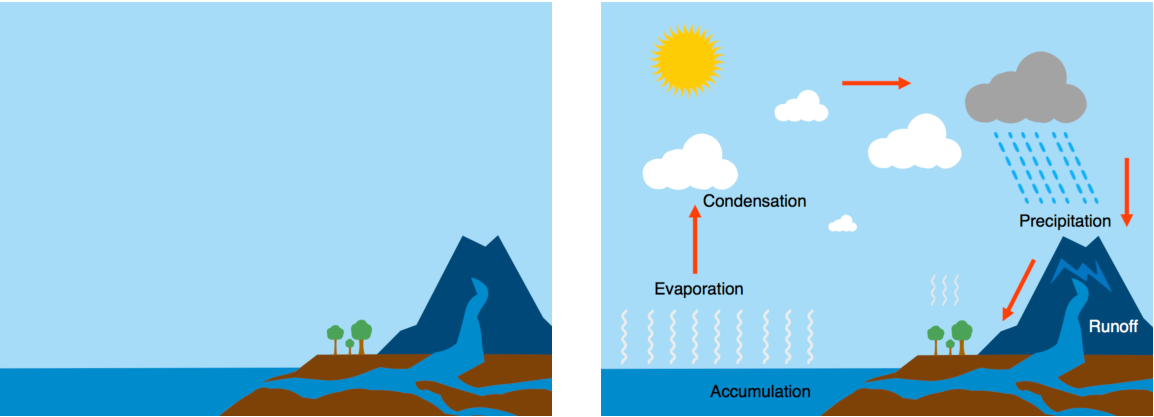
\includegraphics[width=1\columnwidth]{figures/watercycle}
        \caption{Lorem ipsum}
    \end{subfigure}
    ~ 
    \begin{subfigure}[t]{0.48\columnwidth}
        \centering
        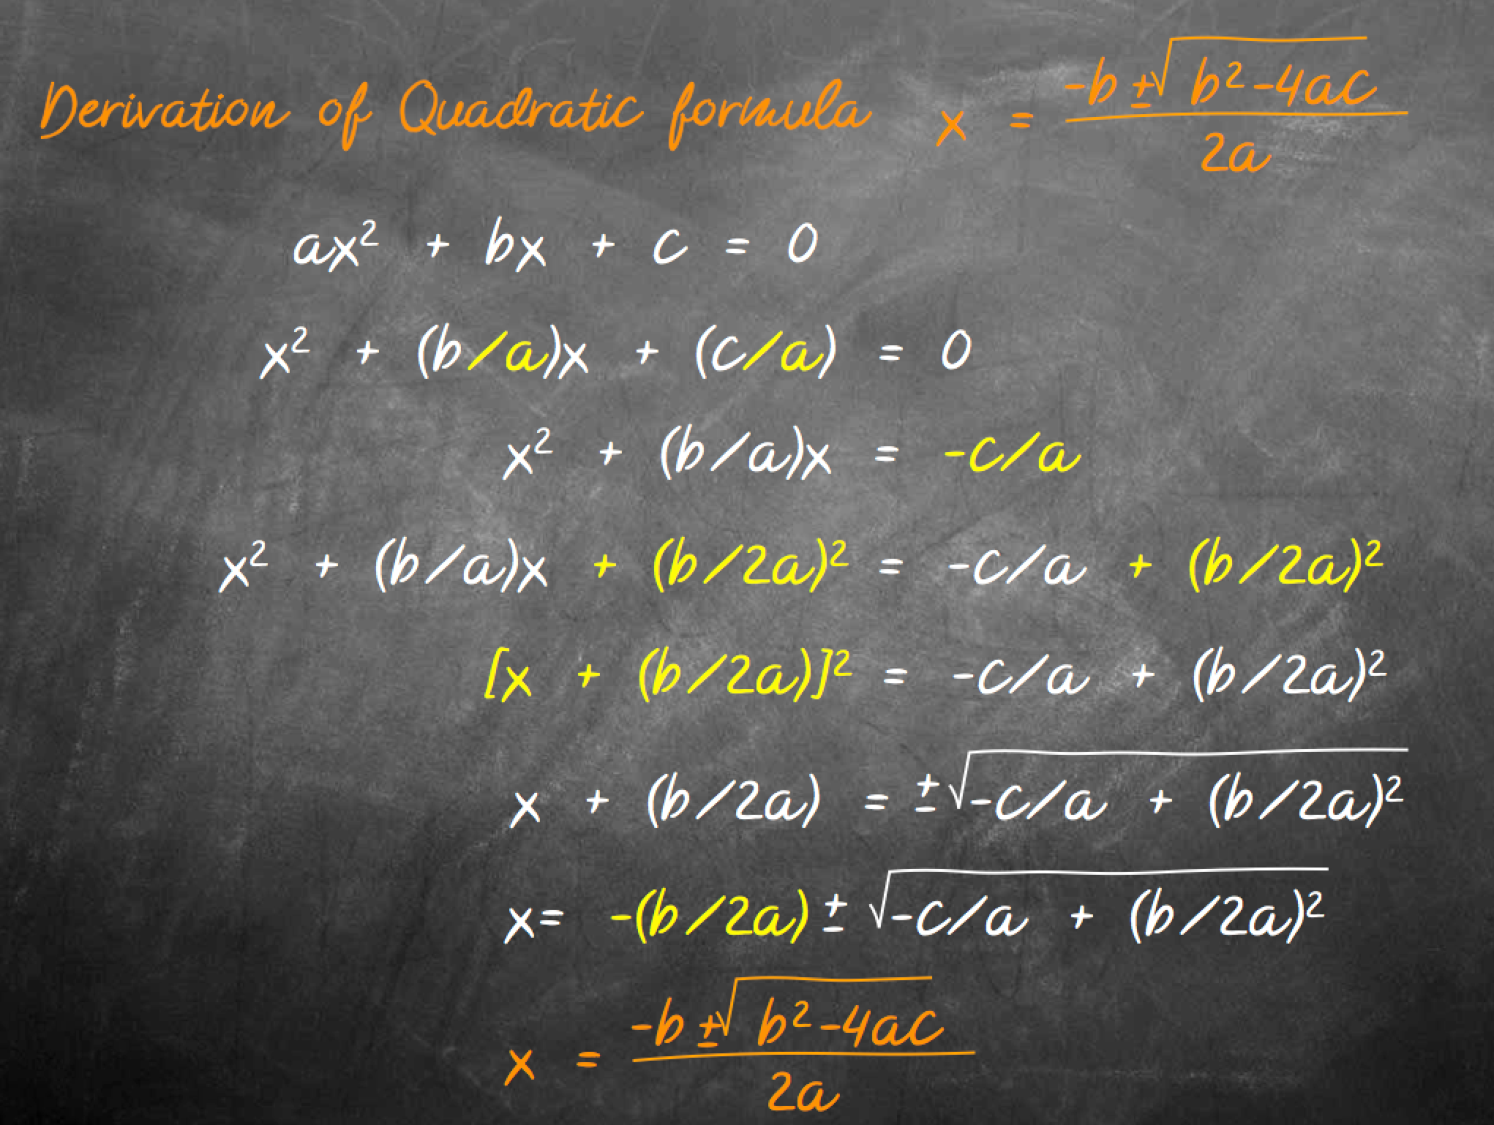
\includegraphics[width=1\columnwidth]{figures/quadformula}
        \caption{Lorem ipsum}
    \end{subfigure}  
    ~
    \begin{subfigure}[t]{0.48\columnwidth}
        \centering
        
\includegraphics[width=1\columnwidth]{figures/tools}
        \caption{Lorem ipsum}
    \end{subfigure}  
    \caption{Evaluation slides}
\end{figure}

We evaluate \interface\ from two perspectives: from the presenter's point of view and from the audience's point of view. 

%\wil{If we have time, it could be useful to include even an informal
%  evaluation of the space manipulation features. Maybe just give users
%  a script that includes explicit ``improvisations'' beyond the
%  prepared content and ask for qualitative feedback?}

\val{Explain that we specifically focus on the delivery stage (vs. authoring).}
To better understand the benefits of our interface, we evaluated \interface against two baselines. The first baseline (\textit{BaselinePPT}) represents conventional electronic slides. We use Microsoft PowerPoint, and allow users to apply animation effects, but disallow inking during presentation. The second baseline (\textit{BaselineInk}) represents plain inking condition. We also use Microsoft PowerPoint, but this time we allow users to only use inking without any animations. 

We hypothesized that different types of content will lend themselves to different presentation styles. We compare three different types of content: (1) a text-centered content, explaining the derivation of the quadratic formula \textit{(Derivation)}, (2) a diagram-centered content, describing the hydrologic cycle  \textit{(WaterDiagram)}, and (3) a typical PPT style content with bullet points and images  \textit{(BulletPoints)}, listing different carpentry tools. Using PowerPoint, we pre-authored a single page slide for each of these content types, and separated the elements on each slide into foreground and background elements.  
\val{Figure of three slides, including explanation of background foreground}

\subsection{Presenter's Perspective}
For each trial, participants were given a slide and asked asked to deliver a presentation with it on one of the interfaces. They received verbal and written explanations of the slide content, and had time to familiarize themselves. They were also given time to set up the slide before the presentation. In the BaselinePPT condition, participants could set animation effects on the foreground elements. For the BaselineInk condition, the slide only contained background elements \val{Figure} and participants received a separate printed copy of the slide containing both background and foreground elements. (The printout was available for all conditions.) Participants could set up by writing contents beforehand. This is analogous to a blackboard lecturer writing on the board the before class. For \interface, participants could set up by either revealing foreground elements or writing on top of the slides ahead of time. 

To simulate a real presentation with an audience, participants were asked to pretend that their presentation was being broadcast live as a webcast. We screen recorded each presentation. At the end of each trial, we showed the recording to the presenter, and asked them to self-rate their own presentation, this time pretending that they were students trying to learn the subject. Presenters also completed a questionnaire about each interface.

We used a within-subject design, where each participant delivered presentations on each interface. We counter-balanced the order of the interfaces and the assignment of the content to interfaces. There were 12 participants in total (ages 21 to 31), all of whom were familiar with the PowerPoint interface. 

\subsection{Audience's Perspective}
We conducted a second study, where a separate set of participants were recruited to vote on the presentations delivered using each interface. Although presenters used pre-authored slides in the first study, they were not forced to follow fixed scripts. Hence, the presentations produced in the first study varied considerably in quality (e.g., length, voice, enthusiasm) depending on the presenter. To minimize the effect of the presenter, one of the authors of this paper produced a new set of presentations using the slides from the first study and following fixed scripts. To minimize author bias, we analyzed the presentations from the first study, and used them as a reference. For example, for the BaselinePPT condition, the granularity and order of animations were reproduced from what the presenters in the first study had. In the BaselineInk condition, we referenced the ordering of the inked contents and the choice of ink colors. We also recorded the presentations in such a way that the silent pauses in between inking periods were similar or shorter than in the first study. Finally, for \interface, we referenced the order of revealing, common ink annotations, and the use of slow tracing versus fast scribbling-like gestures to reveal. In most cases, presenters from the first study employed similar approaches so it was straight-forward to extract common qualities. For the few cases, where participants varied in their approach, we selected an approach that was deemed to produce better quality (e.g., finer-grained animations, use of different ink colors). The final recordings of the presentations from both studies are included in the supplementary material. 

We recruited 36 participants to rate the presentations. For each subject matter, participants watched the recordings of three presentations delivered using each interface (9 presentations in total), and voted for the most engaging presentation. 














